%!TEX root =  tfg.tex
\chapter{Iteración 2: Sistema Climático}

\begin{abstract}
Esta iteración añade la segunda parte del MVP de Scubex: El panel de condiciones meteorológicas y marinas, el usuario puede consultar en tiempo real si una zona es apta o no para bucear antes de meterse al agua.\end{abstract}

% ─────────────────────────────────────────────────────────────────────────────
\section{Características desarrolladas esta iteración}
% ─────────────────────────────────────────────────────────────────────────────

\begin{enumerate}
\item Panel de clima con datos atmosféricos y marinos en tiempo real, evaluación automática de condiciones de buceo y caché de 30 minutos. Ver Tabla~\ref{tab:valorAportadoClima}.
\end{enumerate}

Con el mapa ya operativo desde la iteración anterior, la siguiente pieza del MVP es la información climática: antes de cualquier inmersión, el buceador necesita saber si el mar está en calma. El panel proporciona esa respuesta en un único vistazo, evaluando automáticamente las condiciones sin que el usuario tenga que interpretar valores crudos ni consultar varias fuentes.
% ── Tabla 1: Panel de clima ──────────────────────────────────────────────────
\begin{table*}[htb]
	\centering
	\begin{coolTable}{p{4cm}p{\textwidth-4.5cm}}{2}
{Análisis de valor aportado: Panel de Clima}
\textbf{Propuesta}&Consulta del estado del mar y la atmósfera para el punto marcado en el mapa, con evaluación automática de si las condiciones son aptas para bucear.\\
\midrule
\textbf{Valor}&Un buceador no puede planificar una inmersión sin saber si el mar está en calma. El panel proporciona en un único vistazo los datos que determinan la viabilidad de la salida olas, corriente, visibilidad y tiempo sin que el usuario tenga que consultar varias fuentes ni interpretar valores crudos.\\
\textbf{Coste}&Integración con dos endpoints de Open-Meteo (atmospheric forecast y marine API), ambos gratuitos y sin clave. El único esfuerzo no trivial es definir los criterios de evaluación: qué umbrales y pesos determinan si una condición es buena, tolerable o adversa desde el punto de vista del buceo.\\
\textbf{Opciones}&\textbf{Windy}: mapas muy visuales de viento y oleaje, pero no tiene API pública gratuita para datos en crudo. \textbf{Evaluación manual}: mostrar solo los valores numéricos y dejar que el usuario decida; eliminaba la lógica del servidor pero obligaba al usuario a conocer los umbrales de seguridad.\\
\textbf{Riesgos}&Open-Meteo no ofrece SLA; una caída devuelve error sin datos de clima. Los datos marinos no existen en zonas continentales o bahías cerradas, por lo que esos campos pueden llegar vacíos.\\
\textbf{Deuda técnica}&Solo se muestran condiciones en el instante actual; no hay previsión por horas ni por días. Los umbrales de evaluación son globales e iguales para todos los usuarios, sin distinción entre perfiles (principiante vs. avanzado).\\
	\end{coolTable}
	\caption{Análisis de valor aportado: Panel de Clima\label{tab:valorAportadoClima}}
\end{table*}

\clearpage
% ─────────────────────────────────────────────────────────────────────────────
\section{Diseño}
% ─────────────────────────────────────────────────────────────────────────────

El diagrama UML de la Fig.~\ref{fig:diseno02} muestra las relaciones entre los componentes del sistema climático: controlador, servicio, entidad de caché y los dos clientes de Open-Meteo.

\begin{figure}[htbp]
\begin{center}
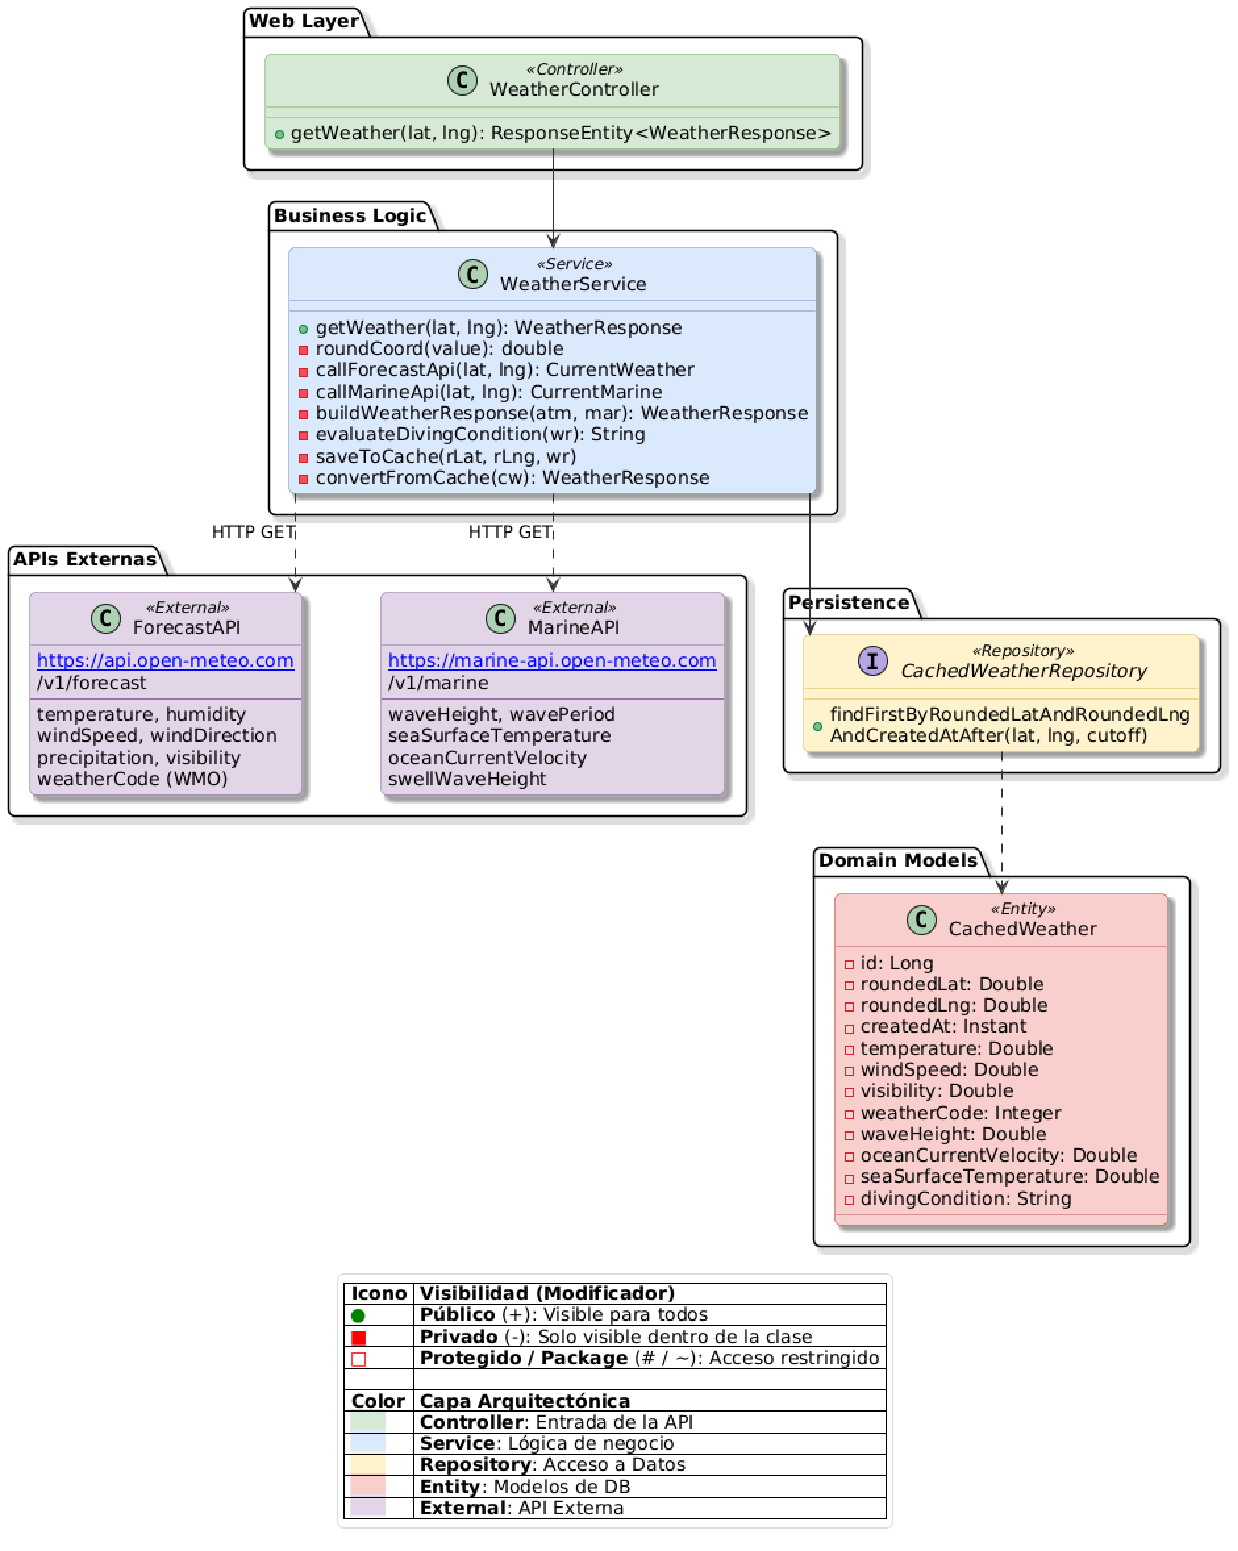
\includegraphics[width=\textwidth]{figures/umlIt2.pdf}
\caption{Diagrama UML de diseño para la iteración 2\label{fig:diseno02}}
\end{center}
\end{figure}

El diseño separa claramente la obtención de datos meteorológicos de la lógica de evaluación de condiciones, lo que permite modificar los criterios de aptitud para el buceo sin tocar la capa de integración con Open-Meteo.

% ───────────────────────────────────────────────────────────────────────────────
\section{Implementación}
% ───────────────────────────────────────────────────────────────────────────────

El sistema climático consulta dos APIs de Open-Meteo para combinar datos atmosféricos y marinos, aplica una puntuación ponderada para determinar si las condiciones son aptas para bucear, y guarda el resultado en caché para evitar llamadas repetidas. Los tres desafíos técnicos y las decisiones adoptadas para resolverlos están recogidos en las tablas siguientes:

\begin{itemize}
    \item \textbf{Dos fuentes de datos} (Tabla~\ref{tab:memo006}): los datos atmosféricos y los marinos provienen de dos endpoints distintos de Open-Meteo; se fusionan en un único objeto de respuesta con tolerancia a que la API marina no tenga datos para la zona.
    \item \textbf{Evaluación automática de condiciones} (Tabla~\ref{tab:memo007}): el usuario necesita saber si puede bucear, no interpretar valores crudos. Se aplica una puntuación ponderada con anulaciones críticas ante los factores más peligrosos.
    \item \textbf{Caché de 30 minutos} (Tabla~\ref{tab:memo008}): el mapa es interactivo y el usuario puede mover el punto libremente; sin caché, cada pequeño desplazamiento generaría dos peticiones a Open-Meteo.
\end{itemize}

\subsection*{Flujo del sistema climático}

Al hacer clic sobre el mapa y activar el panel de clima, el flujo completo es el siguiente:

\begin{enumerate}
    \item El servidor redondea las coordenadas a dos decimales y comprueba si existe un resultado reciente (menos de 30 minutos) para esa zona en base de datos. Si lo hay, lo devuelve directamente sin llamar a ninguna API.
    \item Si no hay caché, consulta la API atmosférica de Open-Meteo: temperatura, humedad, viento, precipitación, visibilidad y código meteorológico WMO.
    \item Consulta la API marina: altura de ola, corriente oceánica, temperatura del agua y oleaje de fondo. En zonas continentales esta llamada devuelve vacío y esos campos quedan sin datos, pero el resto de la respuesta sigue siendo válida.
    \item Los datos de ambas fuentes se fusionan en una única respuesta.
    \item Se evalúan las condiciones de buceo: si algún factor supera un umbral crítico (oleaje~$>$~2{,}5\,m, corriente~$>$~5\,km/h, viento~$>$~40\,km/h, tormenta eléctrica o visibilidad~$<$~1\,000\,m), el resultado es inmediatamente adverso sin calcular la puntuación. En caso contrario, seis factores con pesos distintos determinan si las condiciones son buenas, tolerables o adversas.
    \item El resultado completo se guarda en base de datos bajo las coordenadas redondeadas, con un tiempo de vida de 30 minutos.
    \item La respuesta se devuelve al cliente. Las próximas consultas sobre esa misma zona durante los siguientes 30 minutos se resolverán en el paso~1 sin llamar a ninguna API.
\end{enumerate}

% ── Memorando 006: Doble fuente de datos ─────────────────────────────────────
\begin{table*}[tbp]
	\centering
	\begin{coolTable}{p{4cm}p{\textwidth-4.5cm}}{2}
{Memorando técnico 006: \texttt{WeatherResponse} --- Datos de Dos Fuentes}
\textbf{Asunto}&Los datos atmosféricos y los datos marinos provienen de dos endpoints distintos de Open-Meteo y deben combinarse en una sola respuesta.\\
\midrule
\textbf{Solución}&Ver pasos 2--4 del flujo. Si una de las dos APIs falla o devuelve vacío (por ejemplo, la marina en zonas continentales), esos campos quedan nulos pero el resto de la respuesta sigue siendo válida.\\
\textbf{Motivación}&Tener datos atmosféricos y marinos es la única manera de que el panel sea realmente útil. Separar las dos llamadas permite tolerancia a fallos parciales: si la API marina no tiene datos para una zona interior, el panel sigue mostrando temperatura, viento y lluvia.\\
\textbf{Cuestiones abiertas}&Las dos llamadas se realizan de forma secuencial. Paralelizarlas reduciría la latencia en los casos sin caché.\\
\textbf{Alternativas}&\textbf{Windy Meteo API}: mayor cobertura, pero requiere suscripción de pago.\\
	\end{coolTable}
	\caption{Memorando técnico 006: \texttt{WeatherResponse}\label{tab:memo006}}
\end{table*}

% ── Memorando 007: Evaluación de condiciones ─────────────────────────────────
\begin{table*}[tbp]
	\centering
	\begin{coolTable}{p{4cm}p{\textwidth-4.5cm}}{2}
{Memorando técnico 007: Evaluación Automática de Condiciones de Buceo}
\textbf{Asunto}&El usuario necesita saber si puede bucear, no interpretar una tabla de valores meteorológicos.\\
\textbf{Resumen}&Un algoritmo de puntuación ponderada clasifica las condiciones en \emph{buenas}, \emph{tolerables} o \emph{adversas}, con anulaciones directas ante valores extremos en los factores más críticos.\\
\midrule
\textbf{Solución}&Ver paso 5 del flujo anterior. Las anulaciones críticas se comprueban primero; si no se activa ninguna, seis factores con pesos distintos (oleaje~=~3, corriente~=~3, visibilidad~=~2, viento~=~2, código WMO~=~2, lluvia~=~1) determinan el resultado final.\\
\textbf{Motivación}&El oleaje y la corriente son los factores más peligrosos; por eso tienen el mayor peso y los umbrales de anulación más conservadores. La probabilidad de lluvia tiene el peso mínimo porque no afecta directamente a la seguridad bajo el agua.\\
\textbf{Cuestiones abiertas}&Los umbrales son fijos para todos los usuarios, sin distinción de nivel de experiencia.\\
\textbf{Alternativas}&\textbf{Umbrales fijos sin ponderación}: más simple, pero no refleja que el oleaje siempre importa más que la lluvia.\\
	\end{coolTable}
	\caption{Memorando técnico 007: Evaluación de Condiciones\label{tab:memo007}}
\end{table*}

% ── Memorando 008: Caché de clima ────────────────────────────────────────────
\begin{table*}[tbp]
	\centering
	\begin{coolTable}{p{4cm}p{\textwidth-4.5cm}}{2}
{Memorando técnico 008: Caché de Clima (\texttt{CachedWeather})}
\textbf{Asunto}&Sin caché, cada movimiento del mapa lanzaría dos llamadas a Open-Meteo.\\
\midrule
\textbf{Solución}&Ver pasos 1 y 6 del flujo. Las coordenadas se redondean antes de usarlas como clave de caché (mismo esquema del Memorando~\ref{tab:memo003}), agrupando puntos cercanos bajo la misma entrada.\\
\textbf{Motivación}&El TTL es 30 minutos (frente a las 48 horas del caché de escaneos) porque los datos climáticos cambian más a menudo. Reutilizar el mismo mecanismo de caché en base de datos evita añadir nuevos servicios.\\
\textbf{Cuestiones abiertas}&El caso límite del redondeo (dos puntos muy próximos que caen en celdas distintas) se acepta por la misma razón que en el Memorando~\ref{tab:memo003}: alta complejidad de resolución para bajo impacto.\\
\textbf{Alternativas}&\textbf{TTL más corto (5--10 min)}: más fresco, pero aumenta significativamente las llamadas a Open-Meteo. \textbf{Sin caché}: penaliza la experiencia en sesiones de exploración del mapa.\\
	\end{coolTable}
	\caption{Memorando técnico 008: Caché de Clima\label{tab:memo008}}
\end{table*}

\clearpage
% ─────────────────────────────────────────────────────────────────────────────
\section{Despliegue}
% ─────────────────────────────────────────────────────────────────────────────

Esta iteración no requirió cambios en la infraestructura existente. Open-Meteo es una API pública sin autenticación, por lo que no fue necesario añadir nuevas variables de entorno ni credenciales. La tabla \texttt{cached\_weather} fue creada automáticamente por Hibernate al arrancar el servicio en Railway.

Las URLs de los dos endpoints de Open-Meteo se externalizan en \texttt{application.properties} mediante las propiedades \texttt{open-meteo.weather.url} y \texttt{open-meteo.marine.url}, lo que permite cambiarlas sin recompilar.

% ─────────────────────────────────────────────────────────────────────────────
\section{Pruebas}
% ─────────────────────────────────────────────────────────────────────────────

Las pruebas cubren los tres desafíos técnicos documentados y verifican los pasos clave del flujo del sistema climático.

\subsection*{Sistema climático}

\begin{itemize}
    \item \textbf{Caché activa} (Tabla~\ref{tab:memo008}, paso~1 del flujo): se inyecta una entrada de 10 minutos de antigüedad. Verifica que el servicio devuelve los datos cacheados y no realiza ninguna llamada a Open-Meteo.

    \item \textbf{Anulación crítica por oleaje} (Tabla~\ref{tab:memo007}, paso~5 del flujo): la API marina devuelve oleaje de 3{,}0\,m con condiciones atmosféricas ideales. Verifica que las condiciones de buceo son adversas, confirmando que la anulación crítica se dispara antes de calcular la puntuación ponderada.

    \item \textbf{Zona continental sin datos marinos} (Tabla~\ref{tab:memo006}, pasos~3--4 del flujo): la API marina devuelve cuerpo nulo (coordenadas de Madrid). Verifica que no se lanza excepción, que los campos marinos son nulos y que las condiciones se evalúan correctamente solo con datos atmosféricos.

    \item \textbf{Tolerancia a fallo de la API atmosférica} (Tabla~\ref{tab:memo006}, paso~2 del flujo): la llamada a Open-Meteo atmosférico lanza \texttt{RestClientException}. Verifica que el servicio no propaga el error, que los campos atmosféricos son nulos y que los datos marinos siguen presentes.
\end{itemize}

\begin{quote}
\small\textit{De igual forma que la anterior iteración proyecto cuenta con más pruebas unitarias (controlador de clima, validación de parámetros de entrada) que no se detallan aquí por no estar directamente vinculadas a las decisiones documentadas en esta sección.}
\end{quote}

% ─────────────────────────────────────────────────────────────────────────────
\section{Seguimiento y Control}
% ─────────────────────────────────────────────────────────────────────────────

Esta iteración partió con retraso por el arrastre de la primera, pero resultó más rápida de desarrollar: Open-Meteo ofrece una API bien documentada y no exige cruzar resultados de varias fuentes como el escáner. El trabajo más delicado fue definir cuándo las condiciones son aptas para bucear. Los umbrales de oleaje, viento y temperatura no se pueden fijar con un criterio único y requirieron varias rondas de ajuste con usuarios piloto hasta que el veredicto final resultó coherente con la realidad.

\begin{table*}[htb]
	\centering
	\begin{coolTable}{p{3.5cm}p{3.2cm}p{3.2cm}p{\textwidth-10.4cm}}{4}
{Seguimiento temporal: Iteración 2}
\textbf{Hito}&\textbf{Planificado}&\textbf{Real}&\textbf{Desviación}\\
\midrule
Inicio&23/03/2026&25/03/2026&+2 días (arrastre it.~1)\\
Fin&09/04/2026&12/04/2026&+3 días\\
	\end{coolTable}
	\caption{Seguimiento temporal de la Iteración 2}
\end{table*}

\begin{table*}[tbp]
	\centering
	\begin{coolTable}{p{\textwidth-3.5cm}p{3cm}}{2}
{Desglose de horas: Iteración 2}
\textbf{Actividad}&\textbf{Horas}\\
\midrule
Análisis y diseño del sistema climático&6\\
Integración Open-Meteo atmosférico (backend)&5\\
Integración Open-Meteo marino y datos oceanográficos&5\\
Lógica de evaluación de aptitud para el buceo&4\\
Panel del tiempo (frontend, visualización y condiciones)&12\\
Sistema de caché de 30 minutos (backend)&3\\
Testing y cobertura&3\\
Redacción de la memoria: flujo climático, revisión de umbrales y condiciones de buceo&12\\
\midrule
\textbf{Total}&\textbf{50}\\
	\end{coolTable}
	\caption{Desglose de horas dedicadas en la Iteración 2}
\end{table*}

Todas las características planificadas se completaron. Los 3~días de desviación se deben al ajuste fino de los umbrales de aptitud para el buceo, que requirió varias rondas de validación con condiciones reales antes de que el veredicto resultara coherente.
